\documentclass[a4paper]{article}
\usepackage{zadaci}
\usepackage{wrapfig}
\usepackage{url}
\usepackage{tikz}
\usepackage{amsmath}
\usepackage[normalem]{ulem}
\usetikzlibrary{angles,quotes}
\contestname{Hrvatsko otvoreno natjecanje u informatici\\4.\ kolo, 18. siječnja 2020.}
\markright{\textbf{\textsf{Opisi algoritama}}}

\usepackage{hyperref}
\hypersetup{
colorlinks=true,
linkcolor=blue,
filecolor=magenta,
urlcolor=cyan,
}

\begin{document}

\section*{Opisi algoritama}
Zadatke, testne primjere i rješenja pripremili: Fabijan Bošnjak, Nikola
Dmitrović, Karlo Franić, Marin Kišić, Josip Klepec, Daniel Paleka, Ivan Paljak
i Paula Vidas.  Primjeri implementiranih rješenja su dani u priloženim izvornim
kodovima.

\subsection*{Zadatak: FPS}
\textsf{Pripremio: Karlo Franić}\\
\textsf{Potrebno znanje: naredba učitavanja i ispisivanja}

Za rješenje ovog zadatka potrebno je pretvoriti minute u sekunde $(X \cdot 60)$ te
dobiveni broj sekundi pomnožiti sa brojem FPS-a (sličica u sekundi).

\textit{Programski kod (pisan u \texttt{Python 3}):}

\vspace{-2ex}
\begin{verbatim}
X = int(input())
Y = int(input())
print(X * 60 * Y)
\end{verbatim}

\subsection*{Zadatak: Amazon}
\textsf{Pripremili: Fabijan Bošnjak i Nikola Dmitrović}\\
\textsf{Potrebno znanje: naredba ponavljanja, naredba odlučivanja, pohlepni algoritam}

Riješimo najprije prvi podzadatak u vrijednosti od $10$ bodova u kojem vrijedi
da je broj paketa u skladištu jednak $3$. U tom slučaju jedino je potrebno
znanje naredbe \texttt{if} kojom provjeravamo za svaku kombinaciju nošenja
paketa vrijedi li i prema tome zaključujemo koliko puta se dron mora vratiti u
skladište.

\textit{Programski kod tog dijela zadatka (pisan u \texttt{Python 3}):}

\vspace{-2ex}
\begin{verbatim}
if K[0] + K[1] + K[2] <= N:
  print(1)
elif K[0] + K[1] <= N or K[1] + K[2] <= N:
  print(2)
else:
  print(3)
\end{verbatim}

Nadalje, za idućih $10$ bodova vrijedilo je da su težine svih paketa jednake,
odnosno postoji $M$ paketa težine $K$ u skladištu. Ovdje je bitno primijetiti
kako će dron u svakoj dostavi uzeti jednak broj paketa. Naime, ako dron može
uzeti paket s oznakom $X$ u nizu u svoju dostavu, ali ne uzme, to znači da će
morati uzeti paket $X$ u sljedeću dostavu. Da smo uzeli paket $X$ u trenutnu
dostavu u koju je mogao ići, u sljedećoj dostavi nakon što bi dron uzeo paket
$X+1$ bi težina bila $K$, a budući da ga nismo uzeli težina sljedeće dostave
nakon što dron uzme paket $X+1$ je $2K$. Dakle, optimalno je uzeti maksimalan
broj paketa u trenutnoj dostavi jer se ne isplati prenositi dalje.

Broj paketa po dostavi koje dron može uzeti je jednak \texttt{N // K}, gdje
\texttt{//} predstavlja cjelobrojno dijeljenje. Broj polijetanja drona je onda
jednak \texttt{ceil(M / (broj paketa koje dron može uzeti u jednoj dostavi))},
gdje \texttt{ceil} predstavlja naredbu zaokruživanja na više.

Rješenje za preostalih $10$ bodova je ujedno i rješenje koje rješava sve
dosadašnje podzadatke. Ključna je primjedba koja je već dokazana u gornjem
dijelu teksta, a to je da se uvijek isplati uzeti paket u trenutnu dostavu ako
ga možemo uzeti. Dakle, trebamo samo prolaziti nizom pomoću \texttt{for}-petlje
i zbrajati težinu trenutne dostave, a kada zbroj pređe nosivost $N$, dodati
jedan na rješenje i resetirati zbrajanje trenutne dostave na težinu prvog
paketa u toj dostavi. Na kraju, ako je težina trenutne dostave veća od $0$, to
znači da se u trenutnoj dostavi nalaze neki paketi pa je potrebno dodatno
povećati brojač za jedan.

\subsection*{Zadatak: Pod starim krovovima}
\textsf{Pripremio: Nikola Dmitrović}\\
\textsf{Potrebno znanje: pohlepni algoritam}

Rješenje se zasniva na ideji da tekućinom do vrha redom punimo čaše ovisno o
njihovoj zapremnini, počevši od onih s najvećom. Na taj ćemo način sigurno
oslobodili najviše čaša.

Promotrimo prvo slučaj kada su sve čaše iste zapremnine. U tom je slučaju
svejedno koje čaše punimo do vrha. Sada samo treba odrediti koliko je čaša
potrebno da bi se u njih ulio zbroj svih tekućina po čašama. Jedno od stanja u
čašama možemo simulirati tako da zbroj tekućina razlijevamo redom počevši od
prve čaše pa sve dok ne potrošimo svu tekućinu.

\textit{Programski kod (pisan u \texttt{Python 3}):}

\vspace{-2ex}
\begin{verbatim}
N = int(input())
ukupno = 0
for i in range(N):
  Ti, Zi = map(int, input().split())
  ukupno += Ti
print(N - (ukupno // Zi + (bool(ukupno % Zi))))
for i in range(N):
  if ukupno - Zi > 0:
    print(Zi, end = ' ')
    ukupno -= Zi
  elif ukupno > 0:
    print(ukupno, end = ' ')
    ukupno = 0
  else:
print(0, end = ' ')
\end{verbatim}

U slučaju kada čaše nisu iste zapremnine, nužno je tekućinu prelijevati iz čaša
manje zapremnine u čaše veće zapremnine. Prvo čaše treba sortirati po njihovoj
zapremnini i onda iz manjih prelijevati u veće.

\subsection*{Zadatak: Spiderman}
\textsf{Pripremio: Ivan Paljak}\\
\textsf{Potrebno znanje: matematika, analiza složenosti}

Riješimo najprije jednostavnije varijante zadatka iz odlomka o bodovanju.

Prvu parcijalu vrijednu $14$ bodova moguće je riješiti jednostavnom simulacijom,
odnosno, sa dvije ugnježđene petlje možemo za svaki par nebodera provjeriti
može li Peter s jednog skočiti na drugi. Vremenska složenost ovakvog rješenja
je $\mathcal{O}(N^2)$.

Za dodatnih $14$ bodova bilo je potrebno iskoristiti činjenicu da postoji svega
$2000$ različitih visina među neboderima. Ako za svaku visinu zapamtimo koliko
ima nebodera te visine, zadatak smo u stvari sveli na prethodno opisano
rješenje.  Razlika je samo u tome što nećemo posjetiti svaki par nebodera, već
svaki par različitih visina. Vremenska složenost ovakvog rješenja je
$\mathcal{O}(M^2)$ gdje $M$ predstavlja broj različitih visina među neboderima.

U testnim primjerima vrijednima dodatnih $14$ bodova, vrijedilo je $K = 0$.
Odnosno, sa zgrade visine $h_i$ bilo je moguće skočiti na zgradu visine $h_j$
ako je $h_j$ djelitelj broja $h_i$. Djelitelje nekog broja $x$ možemo relativno
jednostavno pronaći u vremenskoj složenosti $\mathcal{O}(\sqrt{x})$ pa smo time
dobili algoritam vremenske složenosti $\mathcal{O}(N\sqrt{max_H})$. Ako niste
upoznati s popularnim algoritmom koji traži djelitelje nekog broja, savjetujemo
vam da taj algoritam proučite putem
\href{https://www.math.uh.edu/~minru/web/divis2.html}{ove poveznice}.

Za osvajanje svih bodova bilo je moguće blago modificirati prethodno opisani
algoritam (naputak: promatrajte djelitelje broja $h_i - k$), ali ovdje ćemo
iznijeti drugačiji algoritam koji postiže bolju vremensku složenost. Zapitajmo
se: ,,\textit{Sa kojih bismo sve nebodera mogli skočiti na neboder visine
$h_i$}''.  Odgovor je, dakako, sa nebodera visine $K$, $K + h_i$, $K + 2h_i$,
$K + 3h_i$, \dots.  Neka $max_H$ označava visinu najvišeg mogućeg nebodera,
tada na neboder visine $h_i$, zbog prethodnog zaključka, možemo skočiti sa
$\sim \frac{max_H}{h_i}$ nebodera.  Postavlja se pitanje je li algoritam koji
prolazi po svim visinskim kandidatima sa kojih možemo skočiti na svaki od
nebodera dovoljno brz.  Pretpostavimo najgori slučaj gdje su visine svih
nebodera u ulazu različite, odnosno neboderi su visina $1$, $2$, \dots,
$max_H$. Za prvi (najniži) neboder imamo $\sim \frac{max_H}{1}$ kandidata, za
drugi neboder imamo $\sim \frac{max_H}{2}$ kandidata, \dots i konačno za
najviši neboder imamo $\sim \frac{max_H}{max_H}$ kandidata. Odnosno, ukupan
broj kandidata iznosi $\sim max_H \lg max_H$ što je dovoljno dobro za osvajanje
svih bodova na ovom zadatku. Ako vam ovaj zaključak nije
poznat, savjetujemo vam da ponovo proučite analizu vremenske složenosti
Eratostenovog sita ili proučite
\href{https://www.cs.umd.edu/class/spring2016/cmsc351-0101/harmonic.pdf}{ovaj
dokument}.

Ovisno o načinu implementacije, trebalo je dodatno paziti na slučaj kada je
$K=0$ (skakanje na isti neboder).

\subsection*{Zadatak: Holding}
\textsf{Pripremili: Fabijan Bošnjak i Marin Kišić}\\
\textsf{Potrebno znanje: dinamičko programiranje, memorijske optimizacije}

Rješenje prvog podzadatka je dinamika u kojoj je stanje bitmaska. Razradu tog
rješenja prepuštamo čitateljici za vježbu.

Za drugi podzadatak je poznato da $R = N$, što znači da ćemo brojeve na pozicijama
unutar intervala $L$, $L+1$, \dots, $R$ moći mijenjati samo s brojevima na pozicijama od
$1$ do $L-1$ (u ostatku rješenja kada se spomene samo interval se podrazumijeva da
je interval $L$, $L+1$, \dots, $R$). Prva bitna primjedba jest da nikada nećemo nekom
broju mijenjati poziciju više od jednom. Druga važna primjedba, i puno
manje očita od prethodne, jest da je jedino bitno koje smo elemente izabrali za
mijenjanje unutar intervala te koje izvan, a da će neovisno o tome koje
elemente međusobno mijenjamo zbroj potrošenog novca iz Ivičinog džepa ostati
isti. U prijevodu, ako su pozicije brojeva unutar zadanog intervala koje smo
odlučili mijenjati $i$, $j$; a pozicije brojeva izvan intervala koje smo odlučili
mijenjati $l$, $k$; posve je svejedno hoće li se zamijeniti $i$,$k$ te $j$,$l$ ili $i$,$l$ te
$j$,$k$. Formalni dokaz te tvrdnje ostavljamo čitateljici za vježbu.

\begin{figure}[!htbp]
\centering
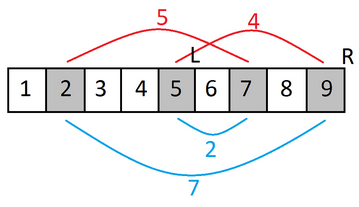
\includegraphics[width=0.4\textwidth]{editorial_holding.png}
\end{figure}

Sada je očigledno jedino bitno odrediti koje elemente biramo unutar intervala
te koje izvan i bitno je da ih je jednak broj. To možemo ostvariti dinamikom $dp$
kojoj su argumenti trenutna pozicija izvan intervala, pozicija unutar intervala
i koliko novaca smo potrošili, a pamti koliko je maksimalno moguće smanjiti
sumu unutar intervala. Početno stanje $dp$ je $dp(1, L, 0)$, a stanje u kojem je
rješenje je $dp(L - 1, R, K)$.
\begin{multline}
  dp(poz_{out}, poz_{in}, spent) = \max \biggl\{ dp(poz_{out} - 1, poz_{in}, spent),
  dp(poz_{out}, poz_{in} - 1, spent),\\
  dp(poz_{out} - 1, poz_{in} - 1, spent - (poz_{in} - poz_{out})) + A[poz_{in}] - A[poz_{out}] \biggr\}
\end{multline}

Prvi prijelaz dinamike govori da ne uzimamo element na poziciji $poz_{out}$, drugi
prijelaz govori da ne uzimamo element na poziciji $poz_{in}$, dok treći govori da
uzimamo oba elementa te ih zamjenjujemo pa zato trošimo $poz_{in} - poz_{out}$
novaca.

Složenost ovog rješenja je $\mathcal{O}(N^2 \cdot K)$.

Taj algoritam je dovoljno brz i za potpuno rješenje, ali ne obuhvaća zamjene s
desne strane intervala jer je $R = N$. Moguće je primjetiti da će se uvijek kao
konačno rješenje uzeti $X$ elemenata s lijeve strane intervala i $Y$ s desne, te $X
+ Y$ elemenata unutar intervala. Očigledno je da ćemo, ako sortiramo pozicije
brojeva unutar intervala koje smo odabrali za zamjenu, prvih $X$ elemenata
zamijeniti s odabranih $X$ s lijeve strane intervala te idućih $Y$ s odabranih $Y$ s
desne strane. To nam daje naslutiti da postoji linija između pozicija unutar
intervala koja određuje da ćemo s lijeve strane te linije sve odabrane brojeve
zamijeniti s odabranim brojevima lijevo od intervala, i obratno za desnu stranu
linije. Zato što mi ne znamo gdje se ta linija nalazi i zato što nama nije
važno koliko se zamjena obavi sa svake strane intervala, već samo potrošen
novac, možemo iskušati gdje se nalazi ta linija za sve pozicije unutar
intervala. To možemo sljedećim linijama koda:

\vspace{-2ex}
\begin{verbatim}
for i in range (L - 1, R+1):
  for j in range (0, K + 1):
    rj = max(rj, dpL(L - 1, i, j) + dpR(R + 1, i + 1, K - j))
\end{verbatim}

Što su $dpL$ i $dpR$? $dpL$ je ona ista dinamika iz prošlog podzadatka, a $dpR$
je posve identična $dpL$ samo što se odvija sa suprotne strane. Još je bitno
napomenuti da je bitno da se po pozicijama unutar intervala kod $dpL$ prelazi
od $L$ prema $R$, a kod $dpR$ od $R$ prema $L$ iz očitih razloga. Složenost
dinamike jest $\mathcal{O}(N^2 \cdot K)$, a spajanja dvaju dinamika
$\mathcal{O}(N \cdot K)$, dakle složenost ovog rješenja je $\mathcal{O}(N^2
\cdot K)$.

Zašto onda to rješenje ne donosi sve bodove? Jer trodimenzionalno polje oblika
\texttt{int dp[N][N][K]} zauzima previše memorije za $N = 100$, ali dovoljno za
$N = 50$.  Dakle još je samo potrebno optimizirati memorijsku složenost. Naime,
ovdje ima više pristupa kako to učiniti, ali vjerojatno najlakši je primjedbom
da će u najgorem slučaju za bilo koji $N$, $L$ i $R$, maksimalna količina novca
potrebna Ivici da izvrši sve moguće promjene biti $\frac{N^2}{4}$. Ako
implemetiramo polje \texttt{int dp[N][N][N*N/4]} to ne prelazi memorijsko
ograničenje od \texttt{256 MiB}. Postoji druga optimizacija koja zamjenjuje
dimenziju $N$ s malom konstantom, ali za implementacijske detalje te
optimizacije proučite službeno rješenje.

\subsection*{Zadatak: Klasika}
\textsf{Pripremio: Ivan Paljak}\\
\textsf{Potrebno znanje: dfs obilazak stabla, stoblo}

Prva dva podzadatka bilo je moguće riješiti više ili manje efikasnom simulacijom
onoga što piše u tekstu zadatka pa ćemo razradu tih algoritama ostaviti
čitateljima za vježbu.

U trećem je podzadatku na svaki upit tipa \texttt{Query} trebalo odgovoriti sa
najduljim putem u stablu koji započinje u danom čvoru $a$. Primijetimo da je
definicija duljine puta pomalo neobična, odnosno, umjesto da zbrajamo duljine
bridova, trebamo koristiti operaciju \textit{xor}. Označimo sa $d(x, y)$
duljinu puta od čvora $x$ do čvora $y$. Primijetimo da vrijedi $d(x, y) = d(1,
x)$ \texttt{xor} $d(1, y)$. Ovo svojstvo možemo iskoristiti
tako da za svaki čvor u stablu pamtimo njegovu udaljenost do korijena. Ovo je
lagano održavati usprkos dodavanju novih čvorova u stablo. Kada dođe upit tipa
\texttt{Query a b}, zadatak se zapravo svodi na pronalaženje neke od zapamćenih
udaljenosti koja xorana s udaljenošću $d(1, a)$ daje najveću vrijednost. Radi
se o poznatom problemu kojeg rješavamo strukturom \textit{stoblo} (engl.\
\textit{trie}). Ako niste upoznati s tim problemom, probajte najprije sami
razmisliti kako biste ga riješili koristeći strukturu stoblo, a u slučaju da ne
uspijete, posjetite ovu
\href{https://www.hackerearth.com/practice/notes/lalitkundu95/tutorial-on-trie-and-example-problems/}{poveznicu}.

Rješenje koje osvaja sve bodove je konceptualno veoma slično, jedini nam je
problem što prilikom prolaska po stoblu nismo sigurni nalazimo se u grani
u kojoj živi neki čvor iz podstabla čvora $b$. Zamislimo da su za svaki čvor
poznate vrijednosti \texttt{discovery} i \texttt{finish} koje odgovaraju
trenutku ulaska i izlaska dfs obilaska stabla u tom čvoru. Kada bismo u svakom
čvoru stobla \texttt{discovery} vrijednosti svih čvorova koji žive u tom
podstablu, tada znamo da se po stoblu smijemo kretati samo po čvorovima
u čijim skupovima postoje vrijednosti veće ili jednake \texttt{discovery[b]} i
manje ili jednake \texttt{finish[b]}. Ispada da je sve ovo relativno jednostavno
izvesti. Najprije ćemo (offline) procesirati sve upite tipa \texttt{Add} te
jednim dfs obilaskom odrediti \texttt{discovery} i \texttt{finish} vrijednosti.
Zatim ćemo ponovno proći kroz sve upite. Oni upiti koji dodaju element u stoblo
će po putu dodavati i vrijednost \texttt{discovery[x]} u odgovarajuće skupove, a
ostali će upiti samo paziti da prilikom obilaska stobla ne ulaze u podstabla
koja nemaju čvorove u odgovarajućem intervalu.

\subsection*{Zadatak: Nivelle}
\textsf{Pripremio: Daniel Paleka}\\
\textsf{Potrebno znanje: metoda kliznog prozora, metoda dva pokazivača}

Rješenje vremenske složenosti $\mathcal{O}(N^2)$ za svaki podstring računa broj
različitih slova. Ako koristimo tzv. \textit{metodu kliznog prozora}, potrebno
je brojati koliko puta se svako slovo pojavljuje, te primijetiti svaki put kad
se neko slovo počne ili prestane pojavljivati. Za detalje implementacije
pogledajte sporije službeno rješenje.

Primijetimo da brojnik izraza koji želimo minimizirati, tj. broj različitih
znakova u podstringu, može poprimiti samo vrijednosti $1$, $2$, \dots, $26$.
Stoga, dovoljno je za fiksnu vrijednost brojnika odrediti najduži podniz koji
ima točno taj broj različitih znakova, te usporediti dobivenih $26$ razlomaka.

Jednostavna implementacija za svaki mogući početak podstringa računa najduži
podstring koji sadrži točno $K$ različitih slova. Ako prethodno za svako slovo
i za svaku poziciju izračunamo prvo sljedeće pojavljivanje tog slova, za svaki
početak možemo brzo isprobati $\le 26$ stringova, koji idu “\textit{do prvog
novog slova}”.

\end{document}
%%% Local Variables:
%%% mode: latex
%%% mode: flyspell
%%% ispell-local-dictionary: "croatian"
%%% End:
